
\documentclass[a4paper]{article}
\usepackage{graphicx}
\usepackage{float}
\usepackage[T2A]{fontenc}
\usepackage{multicol} %колонки
\usepackage{setspace} %межстрочный интервал
\usepackage{fancyhdr} %настройки верхнего и нижнего колонтитулов в документе.
\usepackage{hyphenat}
\usepackage{import}
\usepackage{scn}

\newcommand{\RomanNumeralCaps}[1]
    {\MakeUppercase{\romannumeral #1}}

\usepackage{scrextend}
\usepackage{amsmath}
\usepackage{enumitem}
\usepackage{ragged2e}
\usepackage{mathtools}
\usepackage[left=2.5cm,right=2.5cm,top=2.5cm,bottom=2.5cm]{geometry}

\setlist[itemize]{noitemsep, topsep=0pt} % убрать отступы itemize
\pagestyle{fancy}
\fancyhf{} % очищает все верхние и нижние колонтитулы.
\renewcommand{\headrulewidth}{0pt} % remove the header rule
\fancyfoot[C]{\textbf{\thepage}}
\setcounter{page}{225}% настройка нумерации страниц 
\setlength{\columnsep}{0.4cm} % интервал между колонками
\begin{document}
\setlength\parindent{11pt}
\fontsize{10}{11}\selectfont


\setlength\parindent{0pt} % Убрать в самом начале отступ
\begin{multicols}{2}

\setcounter{figure}{4}
\begin{figure}[H] 
  \centering
  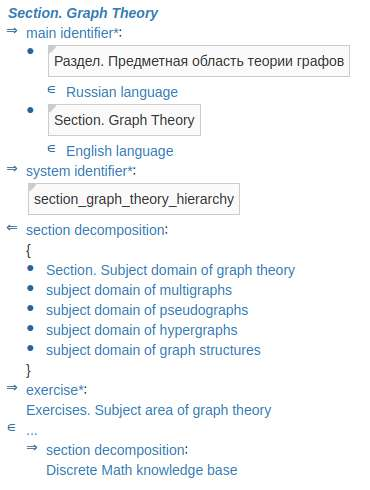
\includegraphics[width=7.5cm]{1.jpg}
  \caption{ Exercise example}
\end{figure}
\begin{itemize}
  \renewcommand{\labelitemi}{1)}
\item Correctness of solved problems is a key aspect when
evaluating a problem solver in discrete mathematics.
This means that the problem solver must be able to
correctly solve any problem in its subject domain.
This includes not only the ability to solve problems,
but also the ability to adapt to different types of
problems and conditions. If there are several ways
to solve a problem, the solver should be able to
choose between them and apply the most appropriate method depending on the specific task conditions. This may involve analyzing the complexity of
different methods, evaluating their effectiveness, and
determining the most optimal approach.
 \renewcommand{\labelitemi}{2)}
\item problem solver in an intelligent tutoring system
should have the ability to describe in detail and stepby-step the process of solving the current problem.
This includes a full or partial description of all
algorithms used, which is critical for students to
understand the logic and methodology of problem
solving.
Describing the problem solving process in detail
helps students understand how to apply theoretical
knowledge in practice. It also helps them develop
critical thinking and analytical skills, as they can
follow the problem solving process and understand
how each step affects the final result.
Describing the algorithms used is also an important
part of the learning process. It helps students understand how different algorithms work and how they
can be applied to solve specific problems. It can also
help them develop programming and algorithmic
thinking skills.
 \renewcommand{\labelitemi}{3)}
\item problem solver in an intelligent tutoring system
should be user-friendly and feature-rich to ensure
effective and productive learning. Usability may
reduce the attractiveness of the problem solver as a
learning tool, as it may increase the time and effort
required to complete tasks, 
and thus  \columnbreak may discourage


users. Multifunctionality is also an important aspect
of a problem solver. This means that a problem
solver should have a wide range of features that can
help users solve different types of tasks. Limited
functionality may make the problem solver less
useful to users, as it may not be able to solve all
types of problems that users encounter.

\vspace{0.2cm}

\end{itemize}

\begin{center} \textit {Intelligent tutoring system for discrete mathematics
problem solver consists of the the following modules:}
\end{center}
\vspace{0.07cm}
\begin{itemize}
    \item module for solving problems;
    \item module for generating and evaluating problem complexity;
    \item module for checking the correctness of the solution.

\end{itemize}

\begin{justify}
In the context of developing a problem solver for
an intelligent tutoring system for discrete mathematics,
multiagent approach can be used to implement different
modules of the system, such as problem solving module,
solution correctness checking module, problems generation and complexity evaluation module and others. Each
module can be represented as an agent that performs its
functions and interacts with other agents to achieve the
goal of the system


  \textbf {Designing a problem solving module.} This module
is part of the intelligent tutoring systems for discrete
mathematics and provides solutions to problems based
on a class of problems.
The functioning of this module consists of the interaction of agents from the following sc-agent hierarchy:
\vspace{0.2cm}








\begin{itemize}
    \item \textbf{Abstract non-atomic SC-agent of problem solving}
    \begin{itemize}
        \item Decomposition of abstract SC-agent
        \begin{itemize}
            \item Abstract SC-agent of task specification generation by template
            \item Abstract SC-agent of solving a complex problem
            \item Abstract non-atomic SC-agent of solving a simple problem
            \begin{itemize}
                \item Decomposition of abstract SC-agent
                \begin{itemize}
                    \item Abstract SC-agent of finding the relation of a given SC-element with a given concept
                    \item Abstract SC-agent of using a unary operation
                    \item Abstract SC-agent of using a binary operation
                \end{itemize}
            \end{itemize}
        \end{itemize}
    \end{itemize}
\end{itemize}





\textbf{Designing a module for generating and evaluating}
problem complexity. This module is an important part
of the intelligent tutoring systems for discrete mathematics and provides problem generation and complexity evaluation. It is a tool that allows the generation of a variety
of problems, taking into account different parameters
and requirements, and at the same time estimating their
complexity in order to adapt problems to the learners’
level of knowledge.
\newpage
Problem generation is an important function of this
module, providing the ability to create tasks using
specified parameters such as problem type, number of
variables, constraints and other factors. This module
generates unique tasks each time, promoting variety and
fun for learners.

~~~Problem difficulty evaluation is another important feature of the module, based on analyzing the generated
problems and determining their difficulty based on specified criteria. The evaluation criteria may include the
number of steps to solve, the use of complex algorithms
or mathematical concepts. Conducting such an evaluation
allows system to objectively assess the complexity of
tasks and compare them.

\textbf{Designing a module for checking the correctness
of the solution.} This module is part of the intelligent
tutoring systems for discrete mathematics and is designed
to check the correctness of the solution of problems. It
analyzes the solution provided by the user and checks if
it corresponds to possible solutions of the problem.
\vspace{0.1cm}


~~The main functions of the module are:
\begin{itemize}
    \item module analyzes the structure of the solution,
checks the presence of the necessary blocks of the
solution, the correctness of their location and links;

    \item module checks the logic of the solution, analyzes
the correctness of algorithms and logical operations
used in problem solving;
    \item module checks the correct syntax of the program
code in the solution;
\item module checks the answer by comparing the obtained result with the expected one and determines
whether the solution is correct or not.
Advantages of the solution correctness checking module:
\item module allows system to automatically analyze the
solution, which significantly speeds up the verification process and reduces the probability of errors;

\item module is based on the specified conditions and
requirements, which allows system to make an objective assessment of the correctness of the solution;

\item module conducts a detailed check of all aspects of
the solution, including structure, logic and syntax,
which allows system to identify and point out errors.
The use of the solution checking module:
\item the user provides their solution in the form of
program code or algorithm;
\item the solution validation module analyzes the provided
solution with using specified algorithms and rules;
\item• the module displays the result of the check, indicating the detected errors or confirming the correctness
of the solution.
\end{itemize}
\vspace{0.3cm}
\begin{center}
    \RomanNumeralCaps{5.}  User interface
\end{center}

The interface for intelligent tutoring systems for discrete mathematics is of particular interest because graphical representation of the main objects of study of
graph theory and set theory, the two main components
of discrete mathematics, graphs and sets, is the most
convenient and effective for human understanding.

~~There are many software solutions related to the visualization of graph and set structures, but most of them are
focused on solving specific highly specialized problems.
In this connection, when it is necessary to solve a new
problem, or conceptually the same problem, but from
another subject area, the development of a new software
solution for the task becomes the only way out, including
the construction of its own visualization.

~~Proceeding from the fact that the most effective learning takes place in practice, when solving specific and
possibly real-life problems, and through the acquisition
of relevant experience, the tutoring system should be
able to provide all the necessary tools and elements of
the graphical interface for the appropriate practice of
learners.

~~In this regard, a virtual space for working with graphs
was developed - an element of the graphical interface,
which contains a graph visualizer and editor, as well as
elements of control and manipulation of graphs. This
interface element allows creating, editing, and loading
graphs stored in the sc-memory of the sc-machine, a
software implementation of the semantic network storage
and processing. In addition, the controls, which are
graphical interpretations of the corresponding elements
of the knowledge base stored in the sc-memory, allow to
perform a certain set of actions on the graphs contained
in the workspace. It is important to note that this set is defined exclusively by the description of the corresponding
actions in the knowledge base, thus ensuring automatic
and dynamic integration of new actions.

~~The graph editor used in the interface was designed
to support the SCg alphabet and behave similarly to the
SCg-editor during user interaction, but many improvements were introduced as well. The following were implemented: moving with touchbar, zooming with "pinch"
on touchbar, etc.

~~In addition, the developed graph editor was designed
in accordance with a modular architecture, where each
element is an independent component responsible exclusively for its functions and extending the capabilities of
the basic graph structure visualization component [11].
Such a solution is particularly time-consuming during
design and initial development, but it allows to extend
the capabilities of the editor in the future using the developed internal programming interfaces for connecting
new components or plug-ins, without any modification of
the source code of the editor or the visualizer. As a result,
the implemented graph editor offers developers interested
in using it not only the simplest and most efficient way
to extend the editor functionality, but also an ability to
customize the editor according to specific requirements,
\newpage
\begin{figure}[H]
    \centering
    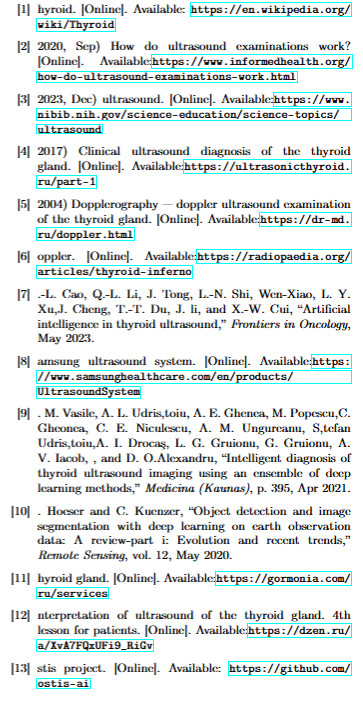
\includegraphics[width=7.5cm]{2.jpg}
    \caption{Graph editor example\label{6}}
 \end{figure}
 \vspace{-5cm}
excluding certain plug-ins built into the editor by default
or changing their configuration.An example of a graph editor is shown in the Figure \ref{6}.

One of the improvements of the graph editor is also a
floating menu, supplied as a plugin (independent component) of the editor as an alternative to the classic menu.
This decision can be justified by the following laws.\\
Fits Law allows to quantify the fact that the farther an
object is from the current cursor position or the smaller
the size of this object, the more time the user will need
to move the cursor to it.\\
Hick’s Law quantifies the observation that the more
options of a given type you provide, the longer it takes
to choose [12].\\
The floating menu appears automatically near the
user’s cursor when selecting certain objects, thereby
minimizing the distance required for the cursor to overcome to perform a particular action on the selected
objects. In addition, the menu is automatically hidden
after receiving a signal indicating cursor movement away
from it, provided that the user has pointed to this menu
at least once, thus informing the user of its existence on
the one hand, but not interfering with the user in his
work on the other hand, conditionally guaranteeing that
the user has paid attention to the existing menu under
the selected objects.\\
An example of the floating menu is shown in the Figure
\ref{7}.
In addition, depending on the type of selected objects
in the floating menu, the system will offer only those
actions that can be performed only on objects of the
selected type. Thus, this solution allows system to significantly reduce the number of options for selecting an
action and, consequently, the time required for the user to
\begin{figure}[H]
    \centering
    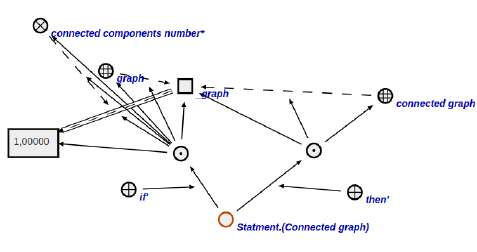
\includegraphics[width=7.5cm]{3.jpg} 
    \caption{ Floating menu exampl\label{7}}
    
 \end{figure}\vspace{-20pt}
\begin{figure}[H]
    \centering
    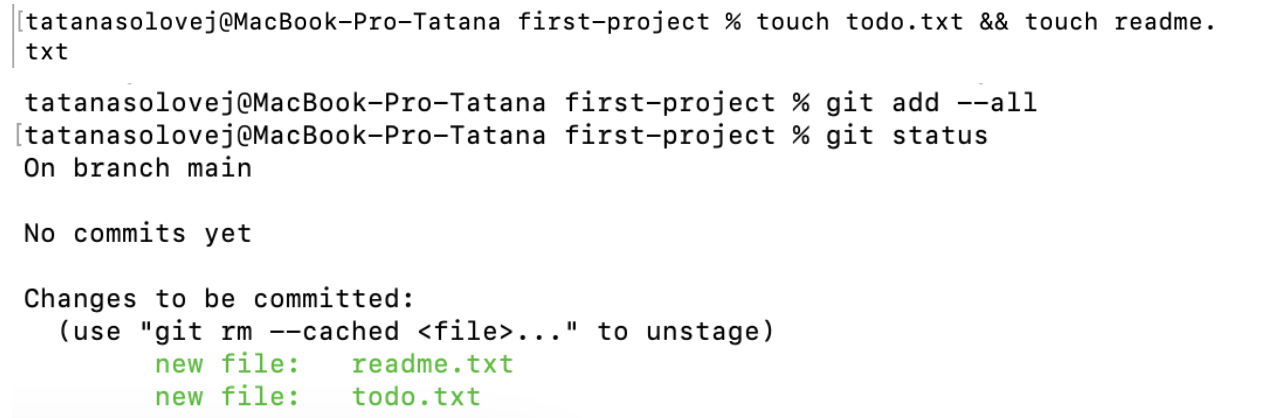
\includegraphics[width=5.5cm]{4.jpg} 
    \caption{ First graph\label{8}}
 \end{figure}\vspace{-20pt}
make a choice, which significantly improves the usability
of the interface.\vspace{-20pt}
\begin{center}
    \RomanNumeralCaps{6.} Demonstration of result
\end{center}\vspace{-20pt}As an example, the problem of determining whether
the union of two graphs, shown in Figure \ref{8} and Figure \ref{9} ,
is a tree is given.\par Figure 10 shows a task template for determining
whether the union of two graphs is a tree. This template
specifies the input arguments of the problem and the goal
of the solution.
\begin{figure}[H]
    \centering
    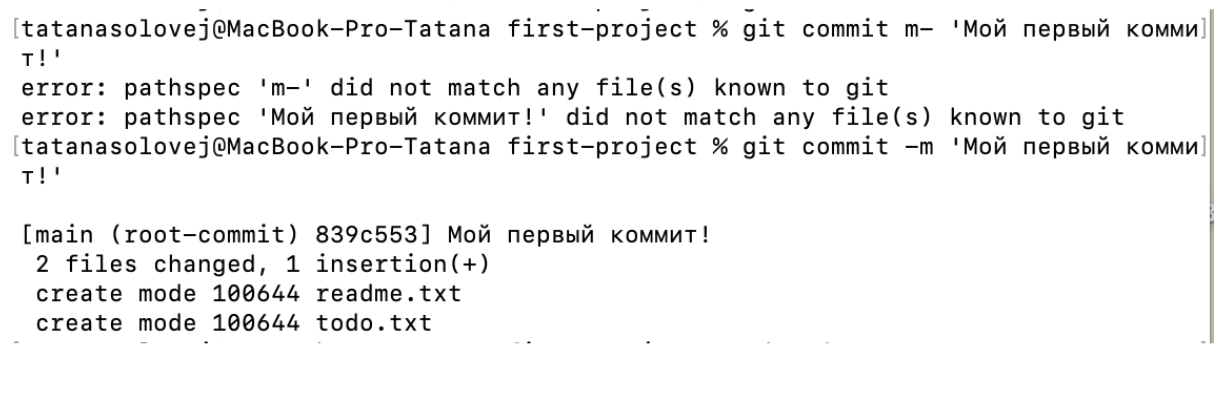
\includegraphics[width=8.5cm]{5.jpg}
    \caption{Second graph\label{9}}
 \end{figure}
\hspace{2cm}
\hspace{10cm}
\end{justify}
\end{multicols}
\end{document}